\chapter{Introducción}
\label{intro} % Etiqueta

\section{Sección Introducción}
$\backslash $newpage agrega una nueva pagina
%\newpage
$\backslash $vfill agrega un espacio para completar
%\vfill
\% para comentar

\subsection{Sub-Sección Introducción}


\section{Nueva Sección Introducción - Listas}

Lista de elementos
\begin{itemize}
	\item Elemento 1
	
	\item Elemento 2
	
	\item Elemento 3
	
\end{itemize}

\section{Ecuaciones}

Puede ir en texto como $x = y + 5$ o en una nueva linea

\[ b + b^2 + b^3 + \dots + b^d + (b^{d+1} - b) =   O(b^{d+1}) \]
\[G = {\{(i, j) \ | \ 0 \leq i \leq N,\ 0 \leq j \leq M \}}\text{.}\]

\section{Imágenes}


\subsection{Una Imagen}

Vemos la imagen de un perro en la Figura \ref{fig:perro}.

\begin{figure}[h]
	\centering %centrada
	
\includegraphics[width=5cm]{images/perro.eps}
	\caption{Imagen de un perro}
	\caption*{{\cite{Bollacker:2008:FCC:1376616.1376746}}}
	\label{fig:perro}
\end{figure}


\subsection{Varias Imágenes}

\begin{figure}[ht]
	
	\centering
	\subfloat[Gato chico \label{fig:gato_chico}]{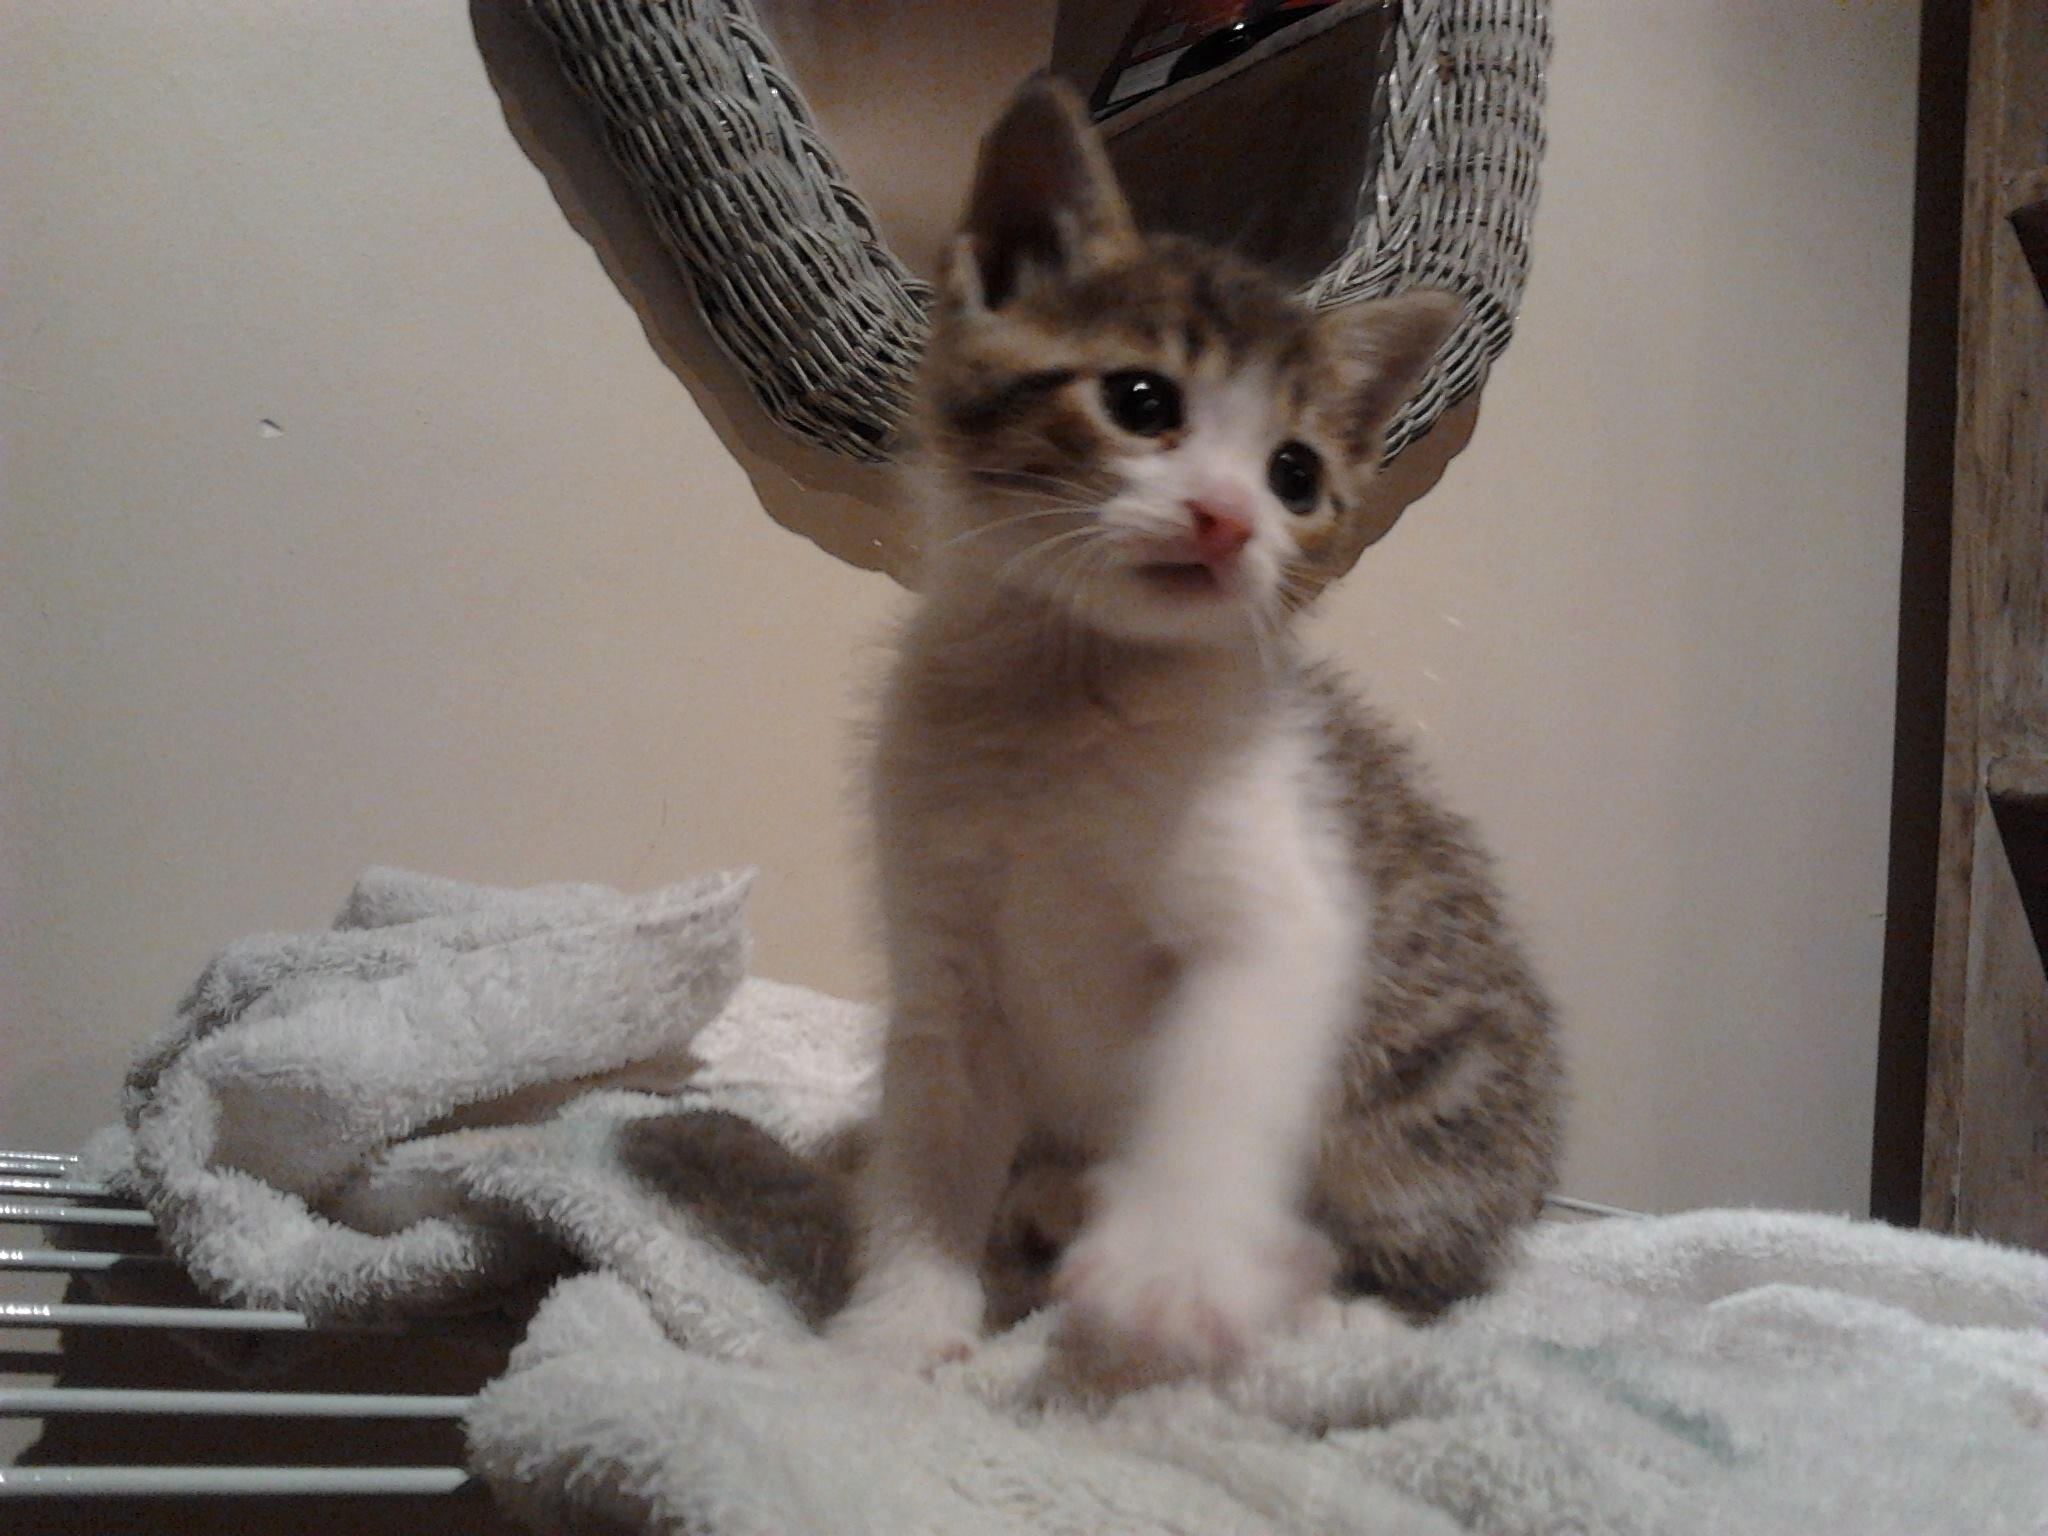
\includegraphics[width = 4cm]{images/gato_chico.eps}}

	%\hspace{\stretch{2}}
	\subfloat[Gato grande \label{fig:gato_grande}]{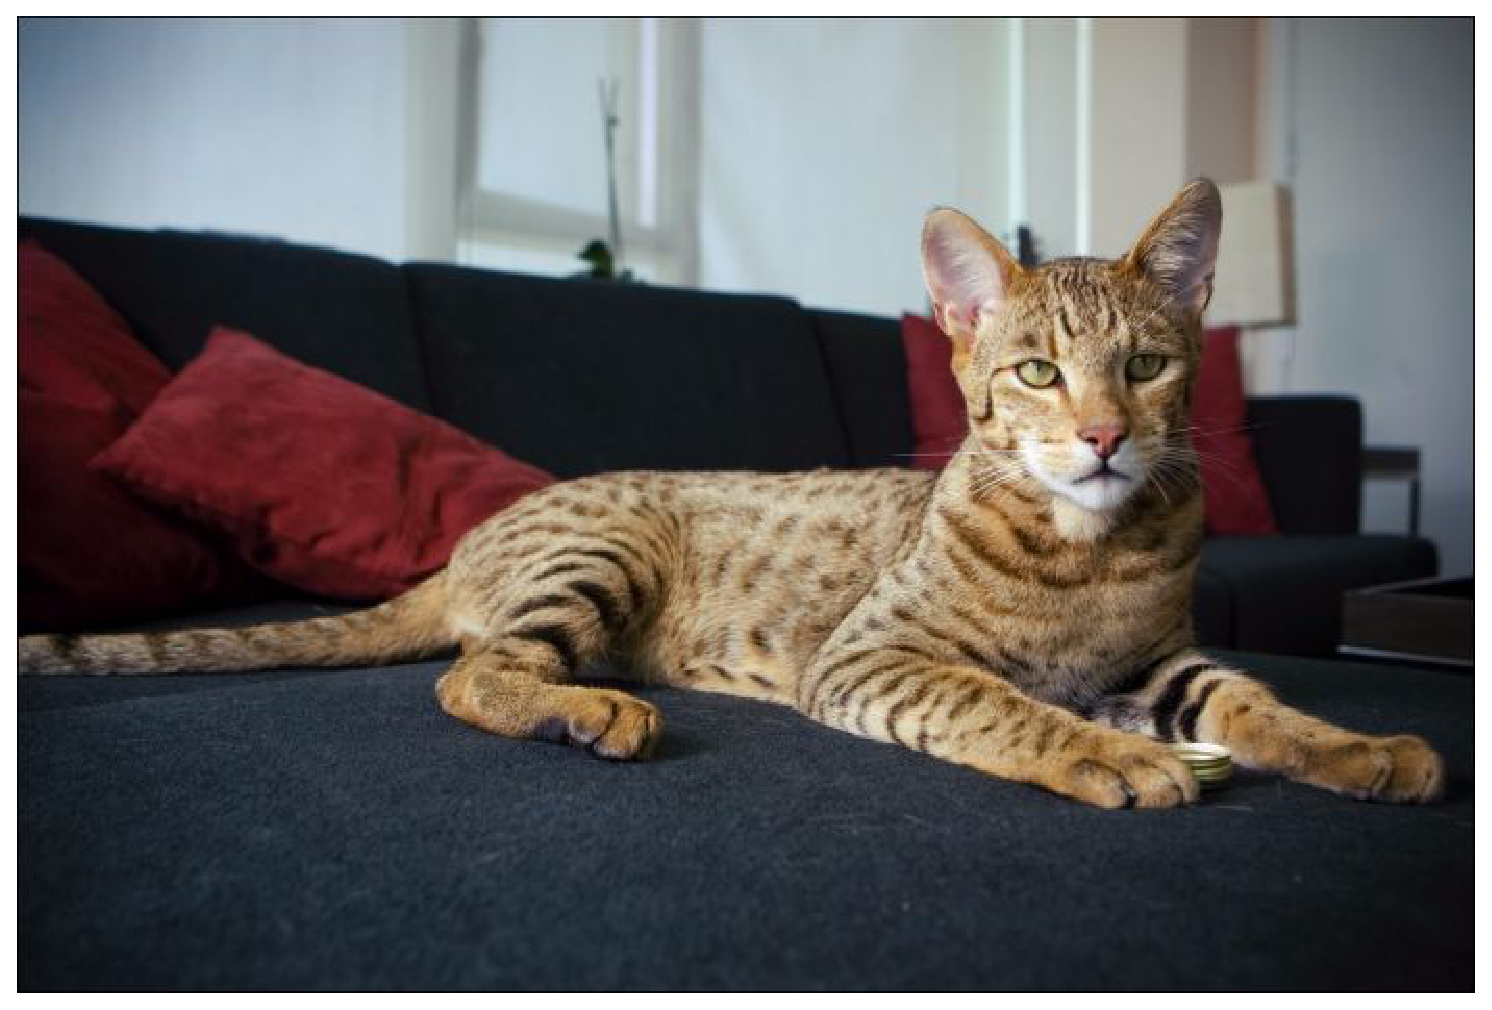
\includegraphics[width = 4cm]{images/gato_grande.eps}}

	%\hspace{\stretch{2}}
	\subfloat[Gato loco \label{fig:gato_loco}]{
\includegraphics[width = 4cm]{images/gato_loco.eps}}
	
	\caption{Diferentes gatos}
	
	\label{fig:Distintos_gatos}
\end{figure}


\section{Referencias}

Para realizar una cita \cite{Bollacker:2008:FCC:1376616.1376746}. Las referencias se encuentran en \textit{referencias.bib}